\chapter{روش انجام پروژه }

در این فصل روش انجام پروژه گفته می‌شود. سامانه پایش شبکه‌های کامپیوتری به ماژول‌های زیر تقسیم می‌شود\cref{fig.11}. ابتدا یک ماژول تحت عنوان هسته \lr{SNMP} در نظر گرفته می‌شود که وظیفه مدیریت پیام‌ها و پیاده‌سازی پروتکل به یک زبان برنامه نویسی خاص است.




\begin{figure}[!h]
\centering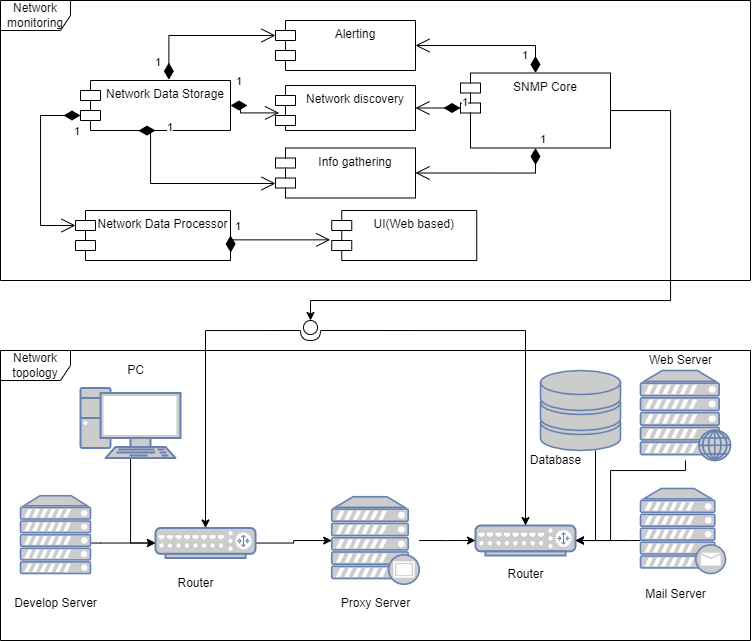
\includegraphics[scale=.55]{./diagram}
\caption{نمودار بلوکی اجزای سامانه}\label{fig.11}
\end{figure}


سپس ماژول کشف عناصر تحت مدیریت شبکه را در نظر گرفته می‌شود، که به کمک ماژول هسته وظیفه جمع آوری اطلاعات ساختاری شبکه را بر عهده دارد. بعد از آن ماژول جمع آوری اطلاعات دستگاه‌های مختلف، عملکرد کل شبکه را رصد می‌کند. حال اگر زمانی با توجه به وجود نوتیفیکیشن‌ها نیاز به هشدار وجود داشت، از ماژول هشدار استفاده می‌شود. 

\newpage

نکته حائز اهمیت در رابطه با سه ماژول آخر این است که هر ماژول از ماژول هسته و همچنین ماژول ذخیره‌سازی اطلاعات شبکه تغذیه می‌شود. همچنین اطلاعاتی که هر ماژول بدست می‌آورد تحویل ماژول ذخیره‌سازی اطلاعات شبکه می‌دهد. در ماژول ذخیره سازی اطلاعات شبکه نیز اطلاعات در پایگاه‌های داده ذخیره می‌شوند، تا برای ماژول پردازشگر اطلاعات شبکه قابل بهره برداری باشد.

در پردازشگر اطلاعات شبکه نیز، اطلاعات خام دریافتی از ماژول ذخیره سازی اطلاعات شبکه پردازش می‌شوند تا اطلاعات قابل فهم توسط مدیر استخراج شود. حال باید اطلاعات تولید شده به ماژول رابط کاربری داده شود.

ماژول رابط کاربری نیز در قالب یک وب سایت و فراهم آوردن یک پنل ورودی مدیر شبکه نیز اطلاعات ساختاری شبکه، پایش شبکه و هشدارها را نمایش می‌دهد. همچنین از طریق آن می‌توان پارامترهای مختلف برای عناصر مختلف تنظیم و اقدام به اسکن کل شبکه کرد.

اما نیاز است که یک رابطی بین شبکه و سامانه مذکور باشد. در شکلی که بررسی شد، سامانه به یک شبکه فرضی از طریق روترهای آن متصل است. در واقع جمع آوری اطلاعات از شبکه و دریافت نوتیفیکیشن‌ها از طریق ماژول هسته \lr{SNMP} امکان پذیر خواهد بود.
